%
% ここから、各章毎に分割したソースファイルを順番に読込
%
\begin{document}
  %
  \maketitle                         % 表紙
  \begin{frame}{はじめに}
  \begin{itemize}[itemsep=2.5ex, leftmargin=3mm]
      \large
      \item[〇] 報告者がCAEを始めたて初心者の時点で(商用コードで)できて

                いたことを、OpenCAEを用いて再現した

      \item[〇] 上記のうち、メッシュ切について日本語で説明している資料が少ないのが残念

      \item[〇] 最近OpenCAEでも簡単に切れるようになった6面体

	        メッシュを中心に、まとめてみた
  \end{itemize}
\end{frame}
          % はじめに
  \begin{frame}{本日の流れ}
  \begin{itemize}
     \item[▶] \highlight[cud_yellow]{目次}
     \begin{itemize}[itemsep=1.3ex, leftmargin=1cm]
       \item[1.] 自己紹介
       \item[2.] 報告者が当時できていたこと
       \item[3.] 本日の例題と以前の勉強会で報告された結果
       \item[4.] あらためて解いてみた
       \item[5.] まとめ
    \end{itemize}
  \end{itemize}
\end{frame}
           % 目次
  %%%
  %%%
  \begin{frame}{本日の流れ}
  \begin{itemize}
     \item[] 目次
     \begin{itemize}[itemsep=1.3ex, leftmargin=1cm]
        \item[▶1.] \highlight[cud_yellow]{ 自己紹介}
        \item[2.] 報告者が当時できていたこと
        \item[3.] 本日の例題と以前の勉強会で報告された結果
        \item[4.] あらためて解いてみた
        \item[5.] まとめ
     \end{itemize}
  \end{itemize}
\end{frame}
           % 
  \begin{frame}{自己紹介}
  \begin{table}[hbtp]
      \begin{tabular}{rl} % 表は項目名を右寄せ、データを左寄せ
      ハンドル名 & ichmy55(いちみーごーごー)で活動してます \\
      職業       & 普段は某企業で構造解析をやってます  \rule[0mm]{0mm}{7mm} \\
      CAE歴      & 10年ほど前から某商用ソフトを使ったCAEに従事 \rule[0mm]{0mm}{7mm} \\
                 & その前は単なるソフト屋でした \\
      情報発信   & Github : {\urlstyle{same} \color{cud_orange}
                             \href{https://github.com/ichmy55/opencae-slides}{@ichmy55}}
                   (本スライドのソースを置いています) \rule[0mm]{0mm}{7mm}\\
                 & Docswell : {\urlstyle{same} \color{cud_orange}
                             \href{https://www.docswell.com/user/ichmy55}{@ichmy55}}
                   (同PDFファイルを置いています) \\
                 & \\
    \end{tabular}
  \end{table}
\end{frame}
    % 自己紹介
  %%%
  \begin{frame}{本日の流れ}
  \begin{itemize}
      \item[] 目次
      \begin{itemize}[itemsep=1.3ex, leftmargin=1cm]
        \item[1.]  {\color{cud_lightgray} 自己紹介}
        \item[▶2.] \highlight[cud_yellow]{ 報告者が当時出来ていたこと }
        \item[3.] 本日の例題と以前の勉強会で報告された結果
        \item[4.] あらためて解いてみた
        \item[5.] まとめ
     \end{itemize}
  \end{itemize}
\end{frame}
           % 
  \begin{frame}{報告者が当時できていたこと}
  \begin{table}[hbtp]
      \caption{報告者が当時できていたこと}
      \begin{tabular}{|r|l|} % 表は項目名を右寄せ、データを左寄せ
          \hline
          形状     & 3次元形状のみ \rule[0mm]{0mm}{7mm} \\
          \hline
          材質     & 線形弾性体のみ \rule[0mm]{0mm}{7mm} \\
          \hline
          メッシュ & 主に4面体、一部 \highlight[cud_lightpink]{6面体}\rule[0mm]{0mm}{7mm} \\
                   &  \\
          \hline
          境界条件 & 変位拘束と荷重(分布or集中) \rule[0mm]{0mm}{7mm} \\
          \hline
          結果処理 & 反力のチェックサム \rule[0mm]{0mm}{7mm} \\
                   & 接点データ外だし→表計算ソフトでグラフ化 \\
          \hline
          \multicolumn{2}{c}{これらをOpenCAEで試してみる}  \rule[0mm]{0mm}{7mm}
    \end{tabular}
  \end{table}
\end{frame}
      % 
  %%%
  \begin{frame}{本日の流れ}
  \begin{itemize}
      \item[] 目次
      \begin{itemize}[itemsep=1.3ex, leftmargin=1cm]
        \item[1.] {\color{cud_lightgray} 自己紹介}
        \item[2.] {\color{cud_lightgray} 報告者が当時出来ていたこと}
        \item[▶3.] \highlight[cud_yellow]{ 本日の例題と以前の勉強会で報告された結果}
        \item[4.] あらためて解いてみた
        \item[5.] まとめ
     \end{itemize}
  \end{itemize}
\end{frame}
           % 
  \begin{frame}{本日の例題}
 
    \begin{columns}[t]
    \begin{column}{0.65\textwidth}
        \\
        <参考文献\cite{wanted} より例題を拝借> \\
	    右\figurename \ref{fig:example-probrem}に示すような圧力容器に内圧10[\si{\mega\pascal}]が \\
        かかっている。
        材料はSB450で、ヤング率は205[\si{\giga\pascal}]、降伏応力は250[\si{\mega\pascal}]である。 \\
        \Erase{本構造は薄肉構造と近似できるとする。} \Add{[後述]}
        \begin{itemize}
          \item[①]{円筒部のA点と半球部のB点の応力状態を求めよ}
          \item[②]{A点とB点ミーゼス相当応力を求め、降伏応力に達する臨界圧力を求めよ}
        \end{itemize}
    \end{column}
    \begin{column}{0.35\textwidth}
      \begin{figure}[htbp]
        \begin{center}
          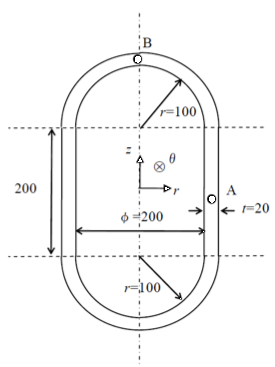
\includegraphics[keepaspectratio,scale=2.2]{images/example-probrem.png}
            \caption{本日の例題(圧力容器)} \label{fig:example-probrem}
        \end{center}
      \end{figure}
    \end{column}
  \end{columns}
\end{frame}
   % 本日の例題と以前の勉強会で報告された結果
  \begin{frame}{以前の勉強会で報告された結果}
 
    \begin{columns}[t]
    \begin{column}{0.7\textwidth}
       <報告者コメント> \\
         ミーゼス応力で比較した結果、A点応力に差異 \\
         \begin{itemize}
            \item[①] 手計算 = 52 [\si{\mega\pascal}]  \\
            \item[②] CAE    = 58.9 [\si{\mega\pascal}]  \\
         \end{itemize}
        <参加者コメント(一部のみ抜粋し要約)> \\
         \begin{itemize}
            \item[①] コンター図がまだら模様でおかしい。\\
                     \Add{メッシュ}に問題がある。 \\
                     正しく計算したければ \highlight[cud_yellow]{6面体メッシュ}で厚み\\
                     方向に4層切りメッシュを作る必要がある。\\
            \item[②] CAE結果と比較する相手として、薄肉構造を仮定 \\
                     % textlint-disable
                     した手計算は相応しくない?
                     % textlint-enable 
	    \item[③] 計算事例(軸対称) <参考文献\cite{Axsymmetric}>
         \end{itemize}
    \end{column}
    \begin{column}{0.3\textwidth}
      \begin{figure}[htbp]
        \begin{center}
          \includegraphics[keepaspectratio,scale=1.5]{images/previous.png}
            \caption{以前の勉強会で報告された結果} \label{fig:previous}
        \end{center}
      \end{figure}
    \end{column}
  \end{columns}
  %
  % TiKZを使った図形の描画 図2でA点を指し示す矢印
  \begin{textblock*}{30pt}(385pt,95pt)
    \begin{tikzpicture}
        \draw[->, draw=cud_red, line width=2pt] (0.7,0.8) -- (0,0.3);
        \node[rectangle,fill=cud_yellow,text width=0.5cm,text centered,rounded corners,minimum height=0.5cm](s) at (1cm,1cm) { \scriptsize A点};
    \end{tikzpicture}
  \end{textblock*}
\end{frame}
 % 以前の勉強会でのコメント
  %%%
  \begin{frame}{本日の流れ}
  \begin{itemize}
      \item[] 目次
      \begin{itemize}[itemsep=1.3ex, leftmargin=1cm]
        \item[1.] {\color{cud_lightgray} 自己紹介}
        \item[2.] {\color{cud_lightgray} 報告者が当時出来ていたこと}
        \item[3.] {\color{cud_lightgray} 本日の例題と以前の勉強会で報告された結果}
        \item[▶4.] \highlight[cud_yellow]{ 改めて解いてみた }
        \item[5.] まとめ
      \end{itemize}
  \end{itemize}
\end{frame}
           % 改めて解いてみた
  \begin{frame}{改めて解いてみた}
  \begin{itemize}
      \item[] 改めて解いてみた
      \begin{itemize}[itemsep=1.3ex, leftmargin=1cm]
        \item[(1)]  今回の改善点
	\item[(2)]  6面体メッシュのすすめ
	\item[(3)]  反力のチェックサム
	\item[(4)]  表計算ソフトでグラフ化
      \end{itemize}
  \end{itemize}
\end{frame}
          % 改めて解いてみた
  \begin{frame}{今回の改善点}
 
    \begin{columns}[t]
    \begin{column}{0.7\textwidth}
        <今回の改善点> \\
         \begin{itemize}
            \item[①] コンター図がまだら模様の件 \\
                     これは4面体メッシュでの解析ではやむを得ない \\
                     \Add{6面体メッシュ}を用いてメッシュを切りなおす
            \item[]
            \item[②] 薄肉構造を仮定した件 \\
                     板厚方向に多くの分割数を確保し \\
                     板厚方向の\Add{応力分布}を\Add{厚肉円筒の応力式}と比較
            \item[]
            \item[③] メッシュ数の節約のため、\\
                     1/8ショートケーキモデルとする
         \end{itemize}
    \end{column}
    \begin{column}{0.3\textwidth}
      \begin{figure}[htbp]
        \begin{center}
          \includegraphics[keepaspectratio,scale=1.5]{work/images/previous.png}
            \caption{以前の勉強会で報告された結果(再掲)}
        \end{center}
      \end{figure}
    \end{column}
  \end{columns}
  %
  % TiKZを使った図形の描画 図2でA点を指し示す矢印
  \begin{textblock*}{30pt}(385pt,95pt)
    \begin{tikzpicture}
        \draw[->, draw=cud_red, line width=2pt] (0.7,0.8) -- (0,0.3);
        \node[rectangle,fill=cud_yellow,text width=0.5cm,text centered,rounded corners,minimum height=0.5cm](s) at (1cm,1cm) { \scriptsize A点};
    \end{tikzpicture}
  \end{textblock*}
\end{frame}
      % 今回の改善点
  \begin{frame}{改めて解いてみた}
  \begin{itemize}
      \item[] 改めて解いてみた
      \begin{itemize}[itemsep=1.3ex, leftmargin=1cm]
        \item[(1)]  {\color{cud_lightgray}今回の改善点}
	\item[▶(2)]   \highlight[cud_yellow]{6面体メッシュのすすめ}
	\item[(3)]  {\color{cud_lightgray}反力のチェックサム}
	\item[(4)]  {\color{cud_lightgray}表計算ソフトでグラフ化}
      \end{itemize}
  \end{itemize}
\end{frame}
          % 改めて解いてみた
  \begin{frame}{あらためてメッシュ要素について復習}
  \begin{table}[hbtp]
    \caption{3次元構造解析で使われる主なメッシュ要素(一部)<参考文献\cite{handbook}>}
    \vspace{-5mm}
    \begin{NiceTabular}{|r|c|c|c|} % 表は項目名を右寄せ、データを中寄せ
       \hline
       名称       & 4面体2次要素 & 6面体1次要素 & 4面体1次要素 \\
       \midrule
       接点配置 &  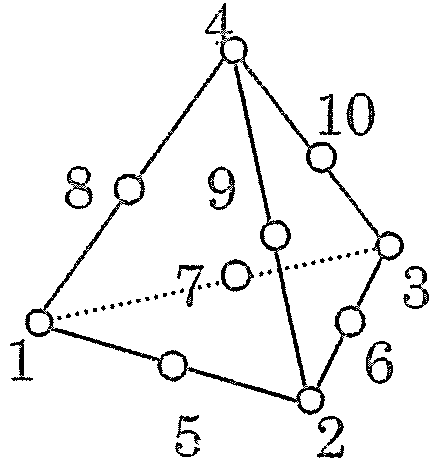
\includegraphics[keepaspectratio,height=35mm]{work/images/tet10.png}
                & 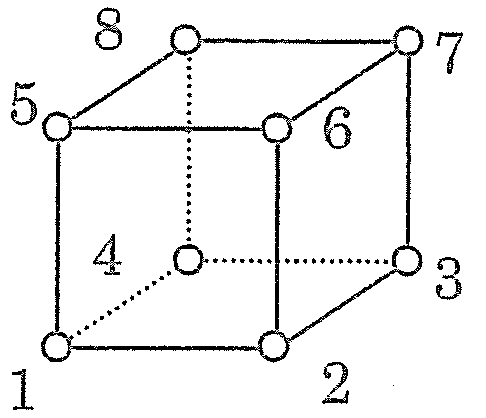
\includegraphics[keepaspectratio]{work/images/hex8.png} 
                & 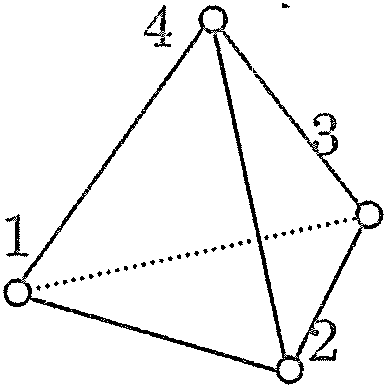
\includegraphics[keepaspectratio]{work/images/tet4.png}  \\
       \hline
       メリット   & 任意の形状で切れる & 見た目が美しい & 接点数節約 \\
       \hline
       デメリット & 多少見た目が悪い   & 形状に人間の介入が必要 & 硬い \\
       \hline
       評価       &   〇               & ◎              & × \\
       \hline
    \end{NiceTabular}
    %
    ※ 他に5面体1次要素(6面体1次要素の面が一つ縮退したもの)もある
    %
    %%% 脚注部 %%%
    %\begin{tablenotes}[para,flushleft,online,normal] %(default:normal)
    %  \item[a] 他に5面体1次要素(6面体1次要素の面が一つ縮退したもの)もある
    %\end{tablenotes}
  \end{table}
  %
  \only<2>{
    % TiKZを使った図形の描画 使用禁止札
    \begin{textblock*}{30pt}(385pt,105pt)
      \begin{tikzpicture}
         \node[rectangle,fill=cud_yellow,text width=0.5cm,text centered,rounded corners,minimum height=0.5cm](s) at (1cm,1cm) { \scriptsize 使用禁止};
      \end{tikzpicture}
    \end{textblock*}
  }
\end{frame}
           % 改めてメッシュについて復習
  \begin{frame}{6面体要素の切り方}
  %
	(1) TransFinite法(以降TF法)
	    
	    ウィキペディアでは、 {\urlstyle{same} \color{cud_orange}
                                   \href{https://ja.wikipedia.org/wiki/マップドメッシュ}
                                   {マップドメッシュ}} として紹介 

	(2) 押し出し法

	(3) イチからスクリプトを用いて作成する
\end{frame}
          % 改めてメッシュについて復習
  %%%
  \begin{frame}{改めて解いてみた}
  \begin{itemize}
      \item[] 改めて解いてみた
      \begin{itemize}[itemsep=1.3ex, leftmargin=1cm]
        \item[(1)]  {\color{cud_lightgray}今回の改善点}
	\item[(2)]  {\color{cud_lightgray}6面体メッシュのすすめ}
	\item[▶(3)]  \highlight[cud_yellow]{反力のチェックサム}
	\item[(4)]  {\color{cud_lightgray}表計算ソフトでグラフ化}
      \end{itemize}
  \end{itemize}
\end{frame}
          % 改めて解いてみた
  \begin{frame}{反力のチェックサム(設定)}
 
  PrePoMaxにおいて、反力チェックサムを確認するには、以下設定する \\
  % 図の挿入
  \begin{figure}[htbp]
    \begin{center}
      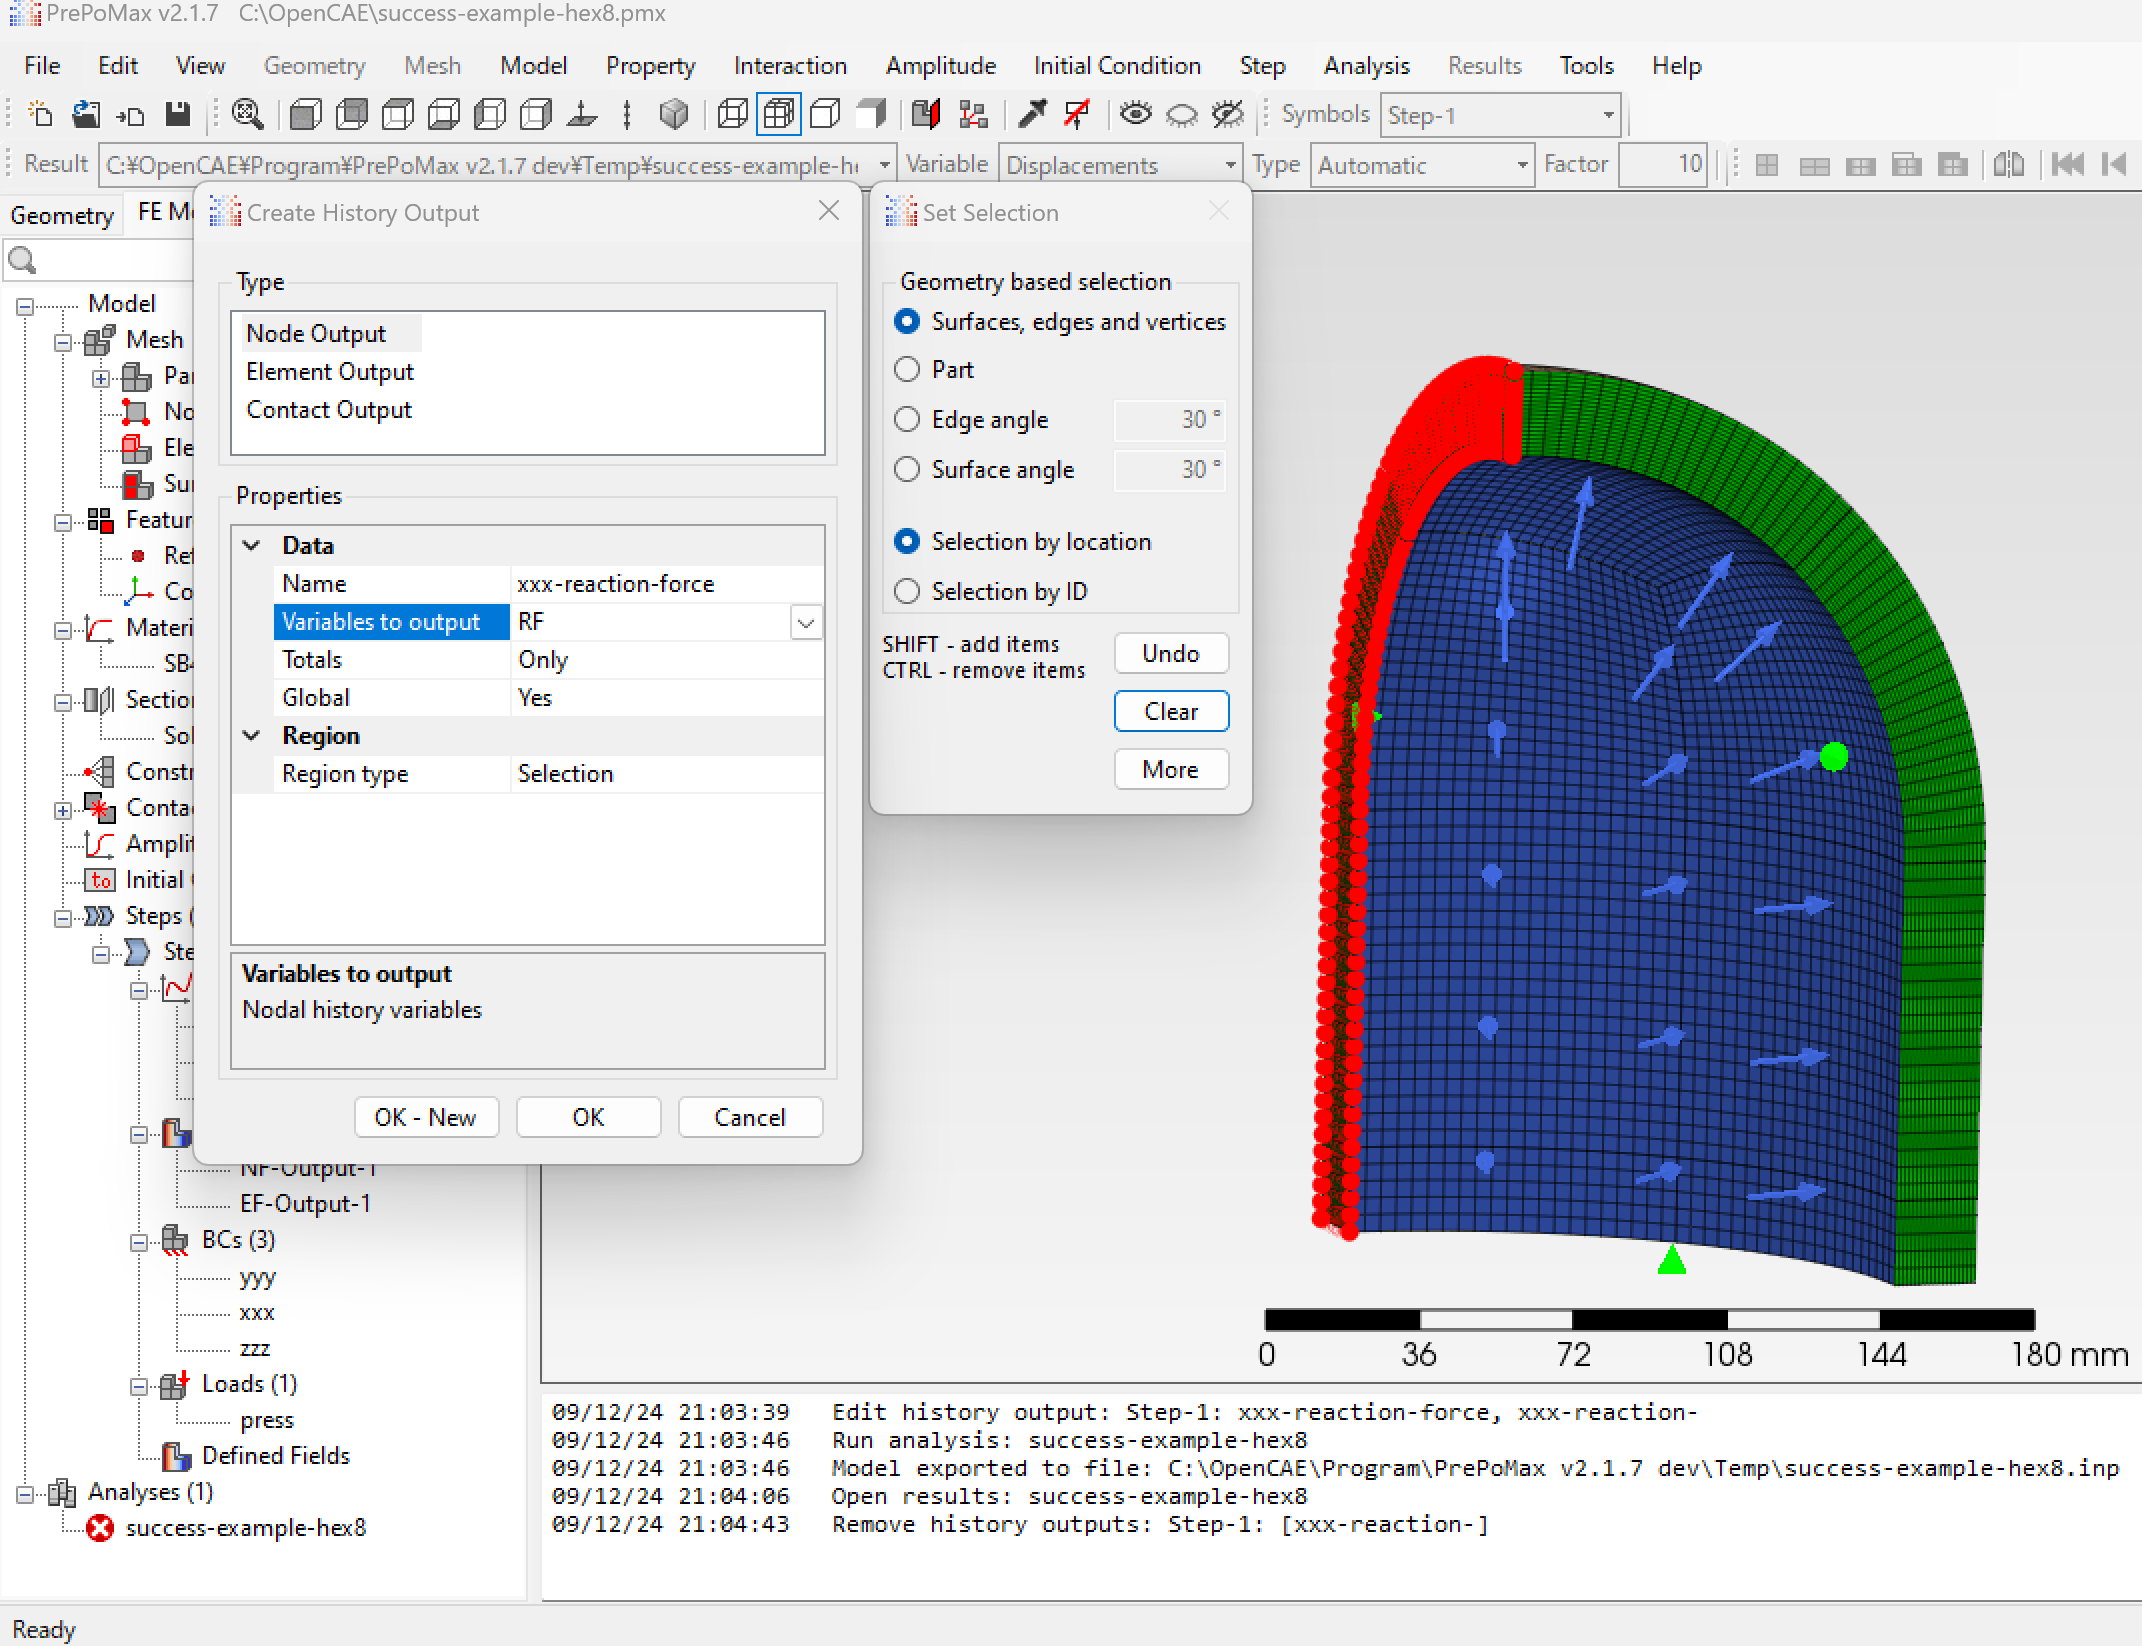
\includegraphics[keepaspectratio,scale=0.285]{work/images/screen01.png}
      \caption{反力チェックサムの設定}
    \end{center}
  \end{figure}
\end{frame}
         % 結果1
  \begin{frame}{反力のチェックサム(結果)}
 
% PrePoMaxにおいて、反力チェックサムを確認するには、以下設定する \\

 % TiKZを使った図形の描画 図2でA点を指し示す矢印
  \begin{textblock*}{0.95\linewidth}(-10pt,-5pt)
    \begin{figure}[htbp]
      \begin{center}
        \begin{tikzpicture}
	  \node [above right,minimum height=50pt, minimum width=420pt,align=left] at (0pt,0pt) {PrePoMaxにおいて、反力チェックサムを確認するには、以下設定する};
          \node[draw=blue,above right,minimum height=70pt,minimum width=110pt,align=left] at (20pt,-60pt)
		{ \scriptsize{合計された結果を見るには}\\
		  \scriptsize{XX-REACTION-FORCEの}\\
		  \scriptsize{TOATALFORCE-RF1のタグを}\\
		  \scriptsize{確認する}};
          \node[above right,minimum height=170pt,minimum width=260pt,align=left] at (130pt,-160pt) {
	    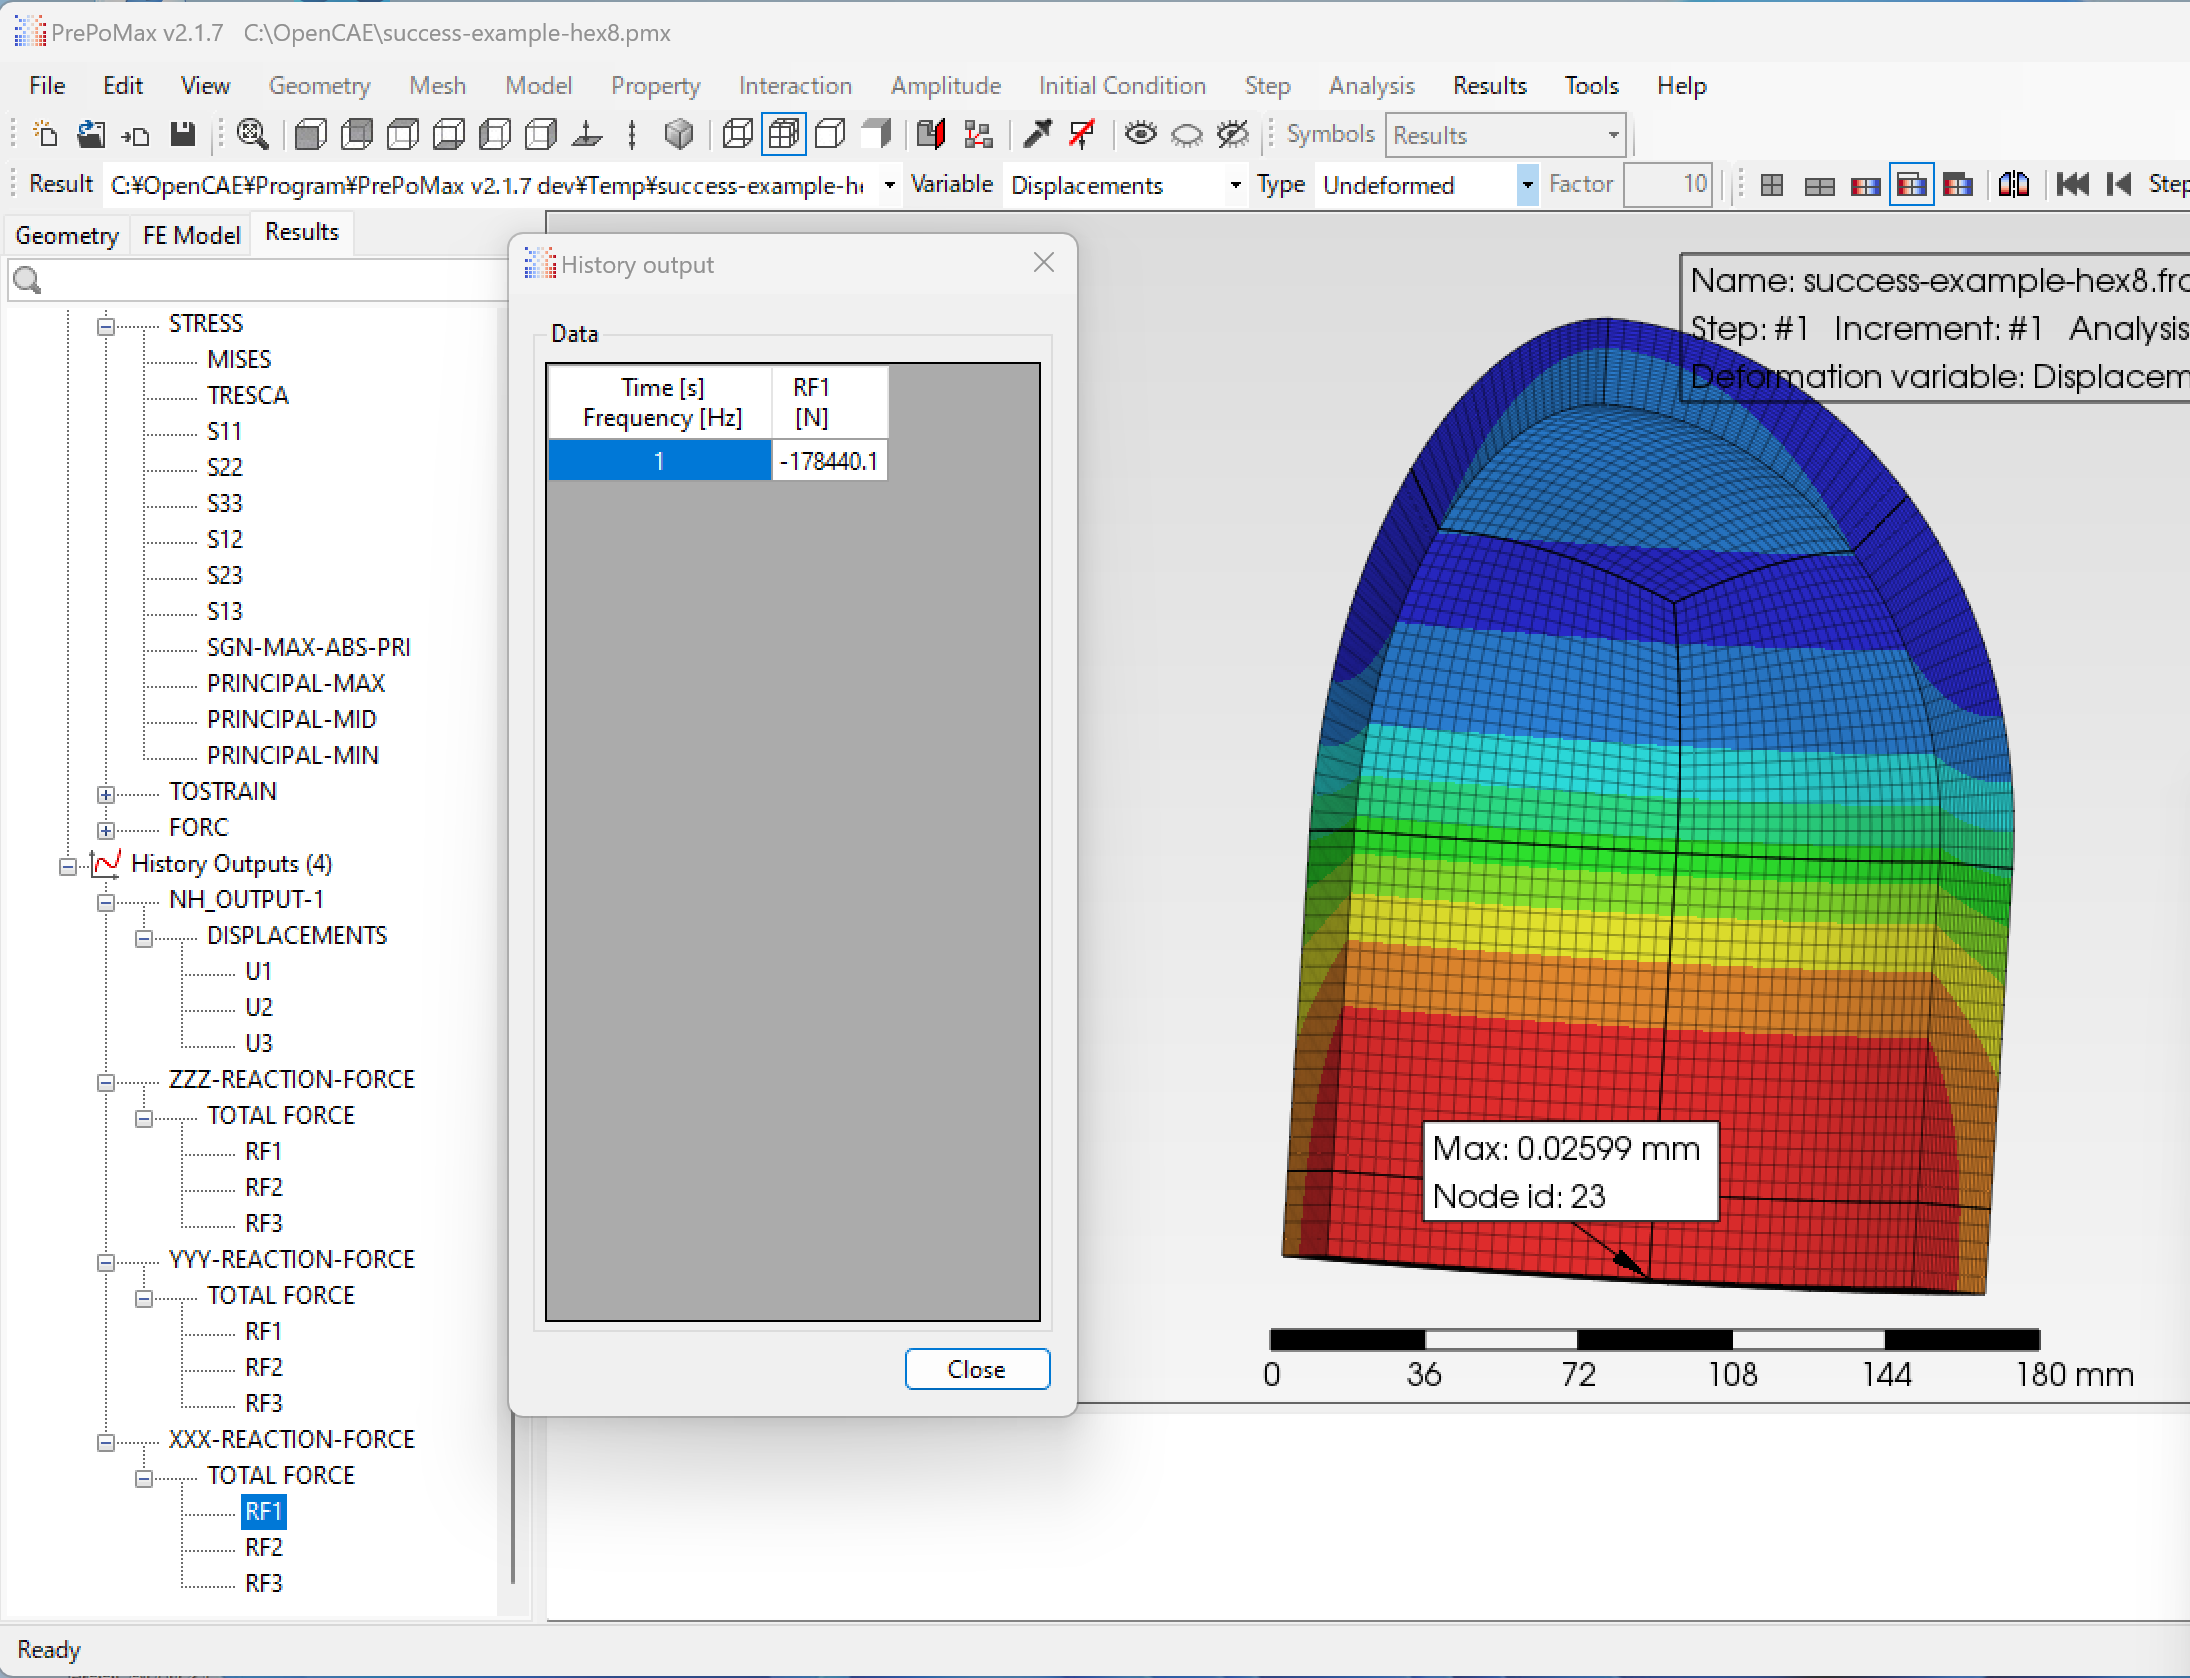
\includegraphics[keepaspectratio,scale=0.265] {work/images/screen02.png}};
          \draw[->, draw=cud_red, line width=1pt] (120pt,-60pt) -- (170pt,-140pt);
          \node[draw=blue,above right,minimum height=70pt,minimum width=100pt,align=left] at (20pt,-160pt)
		{ \scriptsize{この値がX方向から見た}\\
		  \scriptsize{受圧面の投影面積に面圧}\\
		  \scriptsize{をかけたものが}\\
		  \scriptsize{等しいか確認する}\\
		  \scriptsize{今回は誤差0.5\%}};
          \draw[->, draw=cud_red, line width=1pt] (120pt,-120pt) -- (227pt,-35pt);
        \end{tikzpicture}
        \caption{反力チェックサムの確認}
      \end{center}
    \end{figure}
  \end{textblock*}
\end{frame}
         % 結果2
  \begin{frame}{改めて解いてみた}
  \begin{itemize}
      \item[] 改めて解いてみた
      \begin{itemize}[itemsep=1.3ex, leftmargin=1cm]
        \item[(1)]  {\color{cud_lightgray}今回の改善点}
	\item[(2)]  {\color{cud_lightgray}6面体メッシュのすすめ}
	\item[(3)]  {\color{cud_lightgray}反力のチェックサム}
	\item[▶(4)] \highlight[cud_yellow]{表計算ソフトでグラフ化}
      \end{itemize}
  \end{itemize}
\end{frame}
          % 改めて解いてみた
  \begin{frame}{接点応力データの取り出し}
  \begin{textblock*}{0.95\linewidth}(0pt,5pt)
  \begin{figure}[htbp]
    \begin{center}
      % TiKZを使った図形の描画
      \begin{tikzpicture}
	      \node [above right,minimum height=50pt, minimum width=420pt,align=left] at (0pt,20pt) {calculixでは、接点応力データは*.frd ファイルに、接点の選択情報は *.dat \\
	  に出力されるが、これらのファイルは単なるアスキーの数字の羅列ですので、\\
	  メモ帳で必要な行だけ取り出し、表計算ソフトで処理する};
         \node [draw=blue,below right,minimum height=100pt,minimum width=80pt, align=center,fill=cud_lightpink] at (20pt,20pt){全接点情報 \\ *.frd};
         \node [draw=blue,below right,minimum height=40pt,minimum width=80pt,align=center,fill=cud_lightpink] at (20pt,-85pt){指定接点情報 \\ *.dat};
         \node [draw=blue,below right,minimum height=20pt,minimum width=100pt,align=center,fill=cud_lightgray] at (150pt,20pt){接点座標.txt};
         \node [draw=blue,below right,minimum height=20pt,minimum width=100pt,align=center,fill=cud_lightgray] at (150pt,-5pt){要素構成接点.txt};
         \node [draw=blue,below right,minimum height=20pt,minimum width=100pt,align=center,fill=cud_lightgray] at (150pt,-30pt){接点変位.txt};
         \node [draw=blue,below right,minimum height=20pt,minimum width=100pt,align=center,fill=cud_lightgray] at (150pt,-55pt){接点応力.txt};
         \node [draw=blue,below right,minimum height=20pt,minimum width=100pt,align=center,fill=cud_lightgray] at (150pt,-95pt){対象接点.txt};
         \draw[very thick,->] (100pt,10pt)--(150pt,10pt);
         \draw[very thick,->] (100pt,-15pt)--(150pt,-15pt);
         \draw[very thick,->] (100pt,-40pt)--(150pt,-40pt);
         \draw[very thick,->] (100pt,-65pt)--(150pt,-65pt);
         \draw[very thick,->] (100pt,-105pt)--(150pt,-105pt);
         \node [below right,minimum height=20pt,minimum width=100pt,align=center,font=\small] at (75pt,10pt){メモ帳};
         \node [draw=blue,below right,minimum height=140pt,minimum width=30pt, align=center] at (300pt,20pt){表\\計\\算\\ソ\\フ\\ト};
         \draw[very thick,->] (250pt,10pt)--(300pt,10pt);
         \draw[very thick,->] (250pt,-15pt)--(300pt,-15pt);
         \draw[very thick,->] (250pt,-40pt)--(300pt,-40pt);
         \draw[very thick,->] (250pt,-65pt)--(300pt,-65pt);
         \draw[very thick,->] (250pt,-105pt)--(300pt,-105pt);
         \node [below right,minimum height=20pt,minimum width=100pt,align=center,font=\scriptsize] at (225pt,10pt){テキスト\\読込};
         \node [draw=blue,below right,minimum height=140pt,minimum width=30pt, align=center,fill=cud_yellow] at (380pt,20pt){グ\\ラ\\フ\\化};
         \draw[very thick,->] (330pt,-40pt)--(380pt,-40pt);
         \node [below right,minimum height=20pt,minimum width=100pt,align=center,font=\small] at (300pt,-5pt){座標\\変換};
      \end{tikzpicture}
      \caption{接点応力データの取り出し}
    \end{center}
  \end{figure}
	  \end{textblock*}
\end{frame}
         % 結果3
  \begin{frame}{半径方向応力/周方向応力の分布}
 
  半径方向応力については、(最外面、最内面についてはわずかに外れたが) \\
  他は非常によく一致

  周方向応力については、全体的にやや多めに表示されたが、ほぼ一致 
% 図の挿入
\begin{figure}[htbp]
\centering
  \begin{minipage}{0.49\columnwidth}
     \centering
     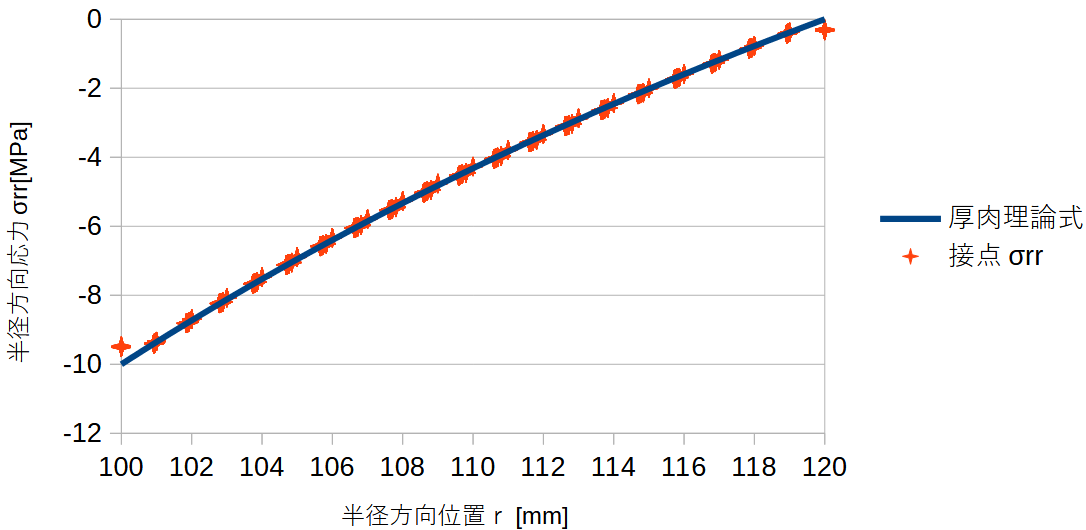
\includegraphics[width=\columnwidth]{images/results01.png}
     \caption{半径方向応力
       \begin{math}
         σ_{rr}
       \end{math}
     }
     \label{fig:hidari}
  \end{minipage}
%
  \begin{minipage}{0.49\columnwidth}
     \centering
     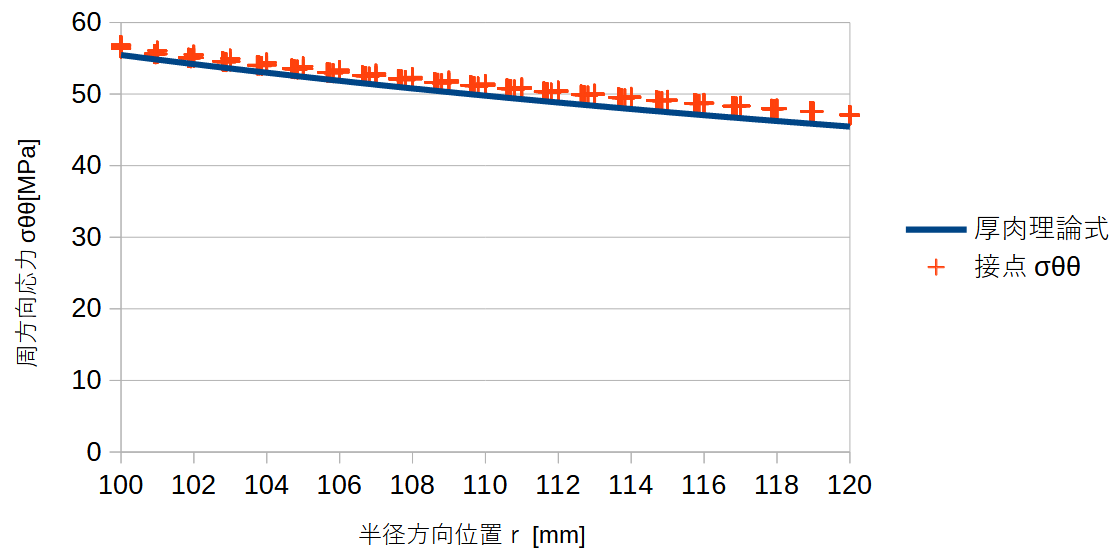
\includegraphics[width=\columnwidth]{images/results02.png}
     \caption{周方向応力
       \begin{math}
         σ_{\theta\theta}
       \end{math}
     }
     \label{fig:migi}
  \end{minipage}
\end{figure}

\end{frame}
         % 結果4
  \begin{frame}{長手方向応力の分布}
 
 長手方向応力については、内面と外面に分布が生じたが、ほぼ一致
% 図の挿入
\begin{figure}[htbp]
\centering
  \begin{minipage}{0.49\columnwidth}
     \centering
     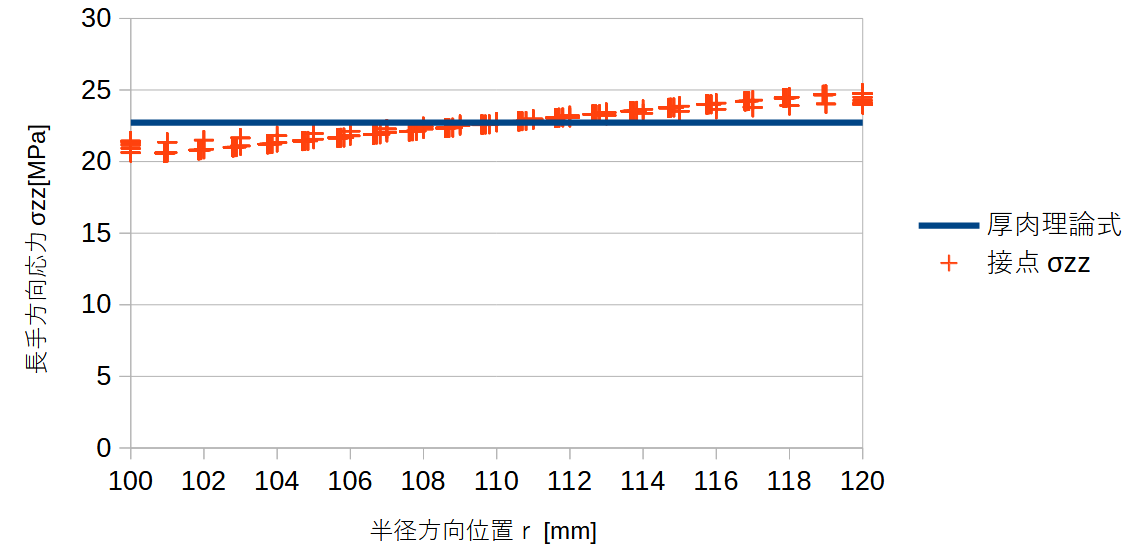
\includegraphics[width=\columnwidth]{images/results03.png}
     \caption{長手方向応力
       \begin{math}
         σ_{zz}
       \end{math}
     }
  \end{minipage}
%
  \begin{minipage}{0.49\columnwidth}
  \end{minipage}
\end{figure}

 全体として、理論式と、ほぼ一致していると言える

\end{frame}
         % 結果5
  %%%
  \begin{frame}{本日の流れ}
  \begin{itemize}
      \item[] 目次
      \begin{itemize}[itemsep=1.3ex, leftmargin=1cm]
        \item[1.] {\color{cud_lightgray} 自己紹介}
        \item[2.] {\color{cud_lightgray} 報告者が当時出来ていたこと}
        \item[3.] {\color{cud_lightgray} 本日の例題と以前の勉強会で報告された結果}
        \item[4.] {\color{cud_lightgray} 改めて解いてみた}
        \item[▶5.] \highlight[cud_yellow]{ まとめ }
      \end{itemize}
  \end{itemize}
\end{frame}
           % 
  \begin{frame}{まとめ}
  \begin{itemize}[itemsep=2.5ex, leftmargin=3mm]
      \large
      \item[〇] OpenCAEは、初級の構造解析者が使えるべき機能を \\
                十分に備えている

      \item[〇] 今回の報告では特にメッシュ切を中心にまとめた

      \item[〇] 次回はメッシュ品質についてまとめる予定

  \end{itemize}
\end{frame}
       % まとめ
  %%%
  \begin{frame}{参考文献}
  % 参考文献リスト
   \beamertemplatetextbibitems
   \bibliographystyle{004-IEEEJtran}
   \bibliography{005-opencae}
\end{frame}
        % 参考文献
  %%%
  \begin{frame}{}
	\scalebox{2}{ご清聴、ありがとうございました}
\end{frame}
           % ご清聴、ありがとうございました
  \begin{frame}[noframenumbering]{付録A. ~今回使用した主なソフト~}
  \begin{table}[hbtp]
    \caption{今回使用した主なソフト}
    \vspace{-7mm}
    \begin{tabular}{|c||l|l|l|} \hline % 表は項目名を中央寄せ、データを左寄せ
	    用途          & 名称 & バージョン & URL \\ \hhline{|=:=|=|=|}
      3次元形状作成 & gmsh & 4.13.1 & {\urlstyle{same} \color{cud_orange}
                                   \href{https://gmsh.info}
				   {gmsh.info}}  \\ \hline
      プリ・ポスト  & PrePoMax & 2.2.3 & {\urlstyle{same} \color{cud_orange}
                                   \href{https://prepomax.fs.um.si/}
				   {prepomax.fs.um.si}}  \\ \hline
      ソルバ(PrePoMax同梱) & Calculix & 2.22 & {\urlstyle{same} \color{cud_orange}
                                   \href{https://calculix.de/}
				   {calculix.de}}  \\ \hline
      表計算        & LibreOffice & 24.8.0.3 & {\urlstyle{same} \color{cud_orange}
                                   \href{https://libreoffice.org/}
				   {libreoffice.org}}  \\ \hline
      OS            & Windows & 11Pro(24H2) & {\urlstyle{same} \color{cud_orange}
                                   \href{https://www.microsoft.com/}
				   {microsoft.com}}  \\ \hline
    \end{tabular}
    \\(注:各ソフトはWindows版x86\_64/amd64用を使用しています)
  \end{table}
\end{frame}
      % 付録 ~今回使用したソフト~
  \begin{frame}[noframenumbering]{付録B. ~ソースのありか~}
  \begin{table}[hbtp]
    \caption{ソースのありか}
    \vspace{-7mm}
    \begin{tabular}{|r||l|l|} \hline % 表は項目名を右寄せ、データを左寄せ
      項目                & 置き場 & URL \\ \hhline{|=:=|=|}
        レジストリ & \multirow{3}{*}{Github} & {\urlstyle{same} \color{cud_orange}
                        \href{https://github.com/ichmy55/opencae-slides}
                         {github.com/ichmy55/opencae-slides}} \\  \cline{1-1} \cline{3-3}
        \multirow{2}{*}{配布物} & & \color{cud_orange}
                         github.com/ichmy55/opencae-slides/releases/ \\
                   & & {\urlstyle{same} \color{cud_orange}
                           \href{https://github.com/ichmy55/opencae-slides/releases/download/v0.2.18/Handout.zip}
                         {releases/download/v0.2.18/Handout.zip}} \\ \hline
        図面       &  Onshape &  {\footnotesize
	                           {\urlstyle{same} \color{cud_orange}
                                     \href{https://cad.onshape.com/documents/8308453c2a5cbbceb286aa1a/w/1773f76374703247baf0d72a/e/bbd26f6d00f1e7f89db44d66}
					{予定地}}(今回報告では未対応)} \\ \hline
        スライド.pdf  & Docswell & {\urlstyle{same} \color{cud_orange}
                                   \href{https://www.docswell.com/user/ichmy55}
                                   {www.docswell.com/user/ichmy55}} \\ \hline
    \end{tabular}
  \end{table}
\end{frame}
      % 付録 ~配布するデータファイル~
  \begin{frame}[noframenumbering]{付録C. ~配布するデータファイル~}
  前ページで示した配布物の中身は以下のとおり
   \begin{table}[hbtp]
    \caption{Handout.zipの中身}
    \vspace{-2mm}
   {\scriptsize
      \begin{tabular}{|c||l|l|l|} \hline % 表は項目名を中央寄せ、データを左寄せ
        ディレクトリ & ファイル種類 & ファイル名 & 概要 \\ \hhline{|=:=|=|=|}
	\multirow{2}{*}{01-gmsh-script} & gmsh入力  & failure-example.geo & メッシュ切失敗形状  \\ \cline{3-4}
				        & スクリプト& successful-example.geo & メッシュ切成功形状  \\ \hline
        \multirow{4}{*}{02-gmsh-shape}  & gmsh形状出力  & failure-example.brep & メッシュ切失敗形状  \\ \cline{3-4}
				        & B-rep形式 & successful-example.brep & メッシュ切成功形状  \\ \cline{2-4}
                                        & gmsh形状出力  & failure-example.step & メッシュ切失敗形状  \\ \cline{3-4}
                                        & step形式  & successful-example.step & メッシュ切成功形状  \\ \hline
        03-prepomax-savefile            & prepomaxセーブ  & success-example-hex8.pmx &   \\ \hline
        04-calculix-input               & calculix入力 & success-example-hex8.inp &   \\ \hline
   \multirow{2}{*}{05-caluculix-output} & \multirow{2}{*}{ocalculix出力}  & success-example-hex8.frd & 全接点応力出力  \\ \cline{3-4}
				        & & success-example-hex8.dat & 特定接点変位出力  \\ \hline
        06-libreoffice                  & 表計算 & successful-example-hex8.ods &   \\ \hline
      \end{tabular}
    }
  \end{table}
\end{frame}
      % 付録 ~ソースのありか~
\end{document}
